%---------- Inleiding ---------------------------------------------------------

\section{Introductie}%
\label{sec:introductie}

In een tijd waarin data als het digitale goud beschouwd wordt, groeit de relevantie van webscraping exponentieel.
Webscraping, een techniek gericht op het geautomatiseerd onttrekken van data van websites, komt voort uit de toenemende 
erkenning van data als drijvende kracht achter zakelijke strategieën, wetenschappelijk onderzoek en artificiële intelligentie.
\\
Bedrijven en organisaties zijn zich steeds meer bewust van de waarde van accurate, actuele data om competitief te blijven
en te anticiperen op veranderende marktomstandigheden. In deze tijd van datagestuurde besluitvorming werkt webscraping als
een krachtige tool om relevevante, real-time data te verkrijgen.
\\
Naast de stijgende behoefte aan gegevens voor zakelijke toepassingen, ondersteunt webscraping ook technologische innovatie. 
De vooruitgang in technologieën zoals artificiële intelligentie, machine learning en big data-analyse vergroot de mogelijkheden
van wat er met de verzamelde gegevens kan worden gedaan.
\\
Binnen deze context is het begrijpen van welke programmeertaal het meest geschikt is voor welke soorten webscraping taken
essentieel. Het doel van deze bachelorproef is een bijdrage leveren aan discussie door Python, Javascript en Java te vergelijken.
Hierdoor kunnen data-engineers en developers een weloverwogen keuze maken bij het implementeren van webscraping projecten
en op die manier optimaal profiteren van de groeiende waarde van data.

%---------- Stand van zaken ---------------------------------------------------

\section{Literatuurstudie}
\label{sec:Literatuurstudie}

De literatuurstudie verkent het domein van webscraping, met specifieke aandacht voor de programmeertalen Python, Javascript en Java,
evenals de verschillende libraries voor deze talen die essentieel zijn voor webscraping scripts.
Deze studie onderzoekt de huidige stand van zaken, richt zich op diverse libraries en identificeert open vragen. 
Deze verkenning vormt de kern van de aankomende vergelijkende studie van programmeertalen en libraries in deze bachelorproef.

\subsection{Webscraping}

\textit{Webscraping}, verwijst naar het automatisch extraheren van informatie en gegevens van websites en deze dan op te slaan in 
in een database of spreadsheet.
Er bestaan een hele hoop webscraping technieken waaronder manuele copy-and paste, matchen van reguliere expressies, HTTP programming
,HTML parsing, DOM parsing, vertical aggregation, webscraping software, semantic notation en computer vision web-page analyserse
\autocite{DeSSirisuriya2015}.

\subsubsection{HTML Parsing}
HTML Parsing houdt in dat de structuur van de HTML documenten wordt geanalyseerd om er specifieke gegevens uit te halen.
Deze techniek werkt het best bij een goed gestructureerde webpagina en maakt gebruik van tags en attributen om de gewenste informatie
te vinden.

\subsubsection{Reguliere exppressies}
Reguliere expressies of regex zijn patronen die gebruikt worden om tekst te matchen op basis van specifieke criteria.
Deze zijn handig voor het zoeken en vinden van informatie met een consistente structuur, zoals telefoonnummers en e-mailadressen.

\subsubsection{API-based webscraping}
Sommige websites bieden Application Programming Interfaces (API's) waarmee gegevens gestructureerd kunnen worden opgevraagd. 
Deze kunnen dus ook gebruikt worden om te webscrapen.

\subsubsection{Selenium}
Selenium is een automatiseringstool waarmee webscraping van dynamische webpagina's mogelijk is, 
waar de inhoud wordt gegenereerd door JavaScript. Selenium simuleert menselijke interactie met een webpagina en is geschikt voor het ophalen van gegevens die via JavaScript worden geladen.

\subsubsection{Machine Learning-based webscraping}
Geavanceerde technieken, zoals 

machine learning, kunnen worden toegepast om webscraping-modellen te trainen voor het herkennen 
van patronen en het extraheren van specifieke informatie. Het grote voordeel dat webscrapen met Machine Learning met zich meebrengt
is dat het flexibel is en zich makkelijker kan aanpassen aan veranderende webpaginastructuren.

\subsubsection*{}
De keuze van de juiste techniek hangt af van een aantal factoren, waaronder de complexiteit van de webpagina's 
die moeten worden gescraped, de hoeveelheid gegevens die moeten worden geëxtraheerd en de beschikbare middelen.

\subsection{Programmeertalen}
De vergelijking van programmeertalen voor webscraping vormt de kern van deze bachelorproef. 
Door de specifieke kenmerken en mogelijkheden van Python, JavaScript en Java te onderzoeken, 
streven we ernaar inzicht te verkrijgen in welke taal het meest geschikt is voor verschillende webscraping-taken. 
Elk van deze programmeertalen heeft zijn eigen ecosysteem van libraries, frameworks en tools die kunnen worden toegepast 
bij het ontwikkelen van webscrapers.

\subsubsection{Python}
Python staat bekend als een van de meest populaire programmeertalen voor webscraping. Het heeft een uitgebreide gemeenschap en
een overvloed aan beschikbare libraries zoals Beautiful Soup en Scrapy~\autocite{Saabith2019}. De eenvoudige en leesbare syntax van Python maakt het 
gemakkelijk voor zowel beginners als ervaren ontwikkelaars om webscraping-scripts te schrijven.

\subsubsection{Javascript}
Javascript, als de dominante programmeertaal op het web, vindt breed gebruik in zowel client-side als server-side webscraping~\autocite{Raval2023}.
Met bibliotheken zoals Puppeteer wordt client-side scraping mogelijk door automatisering van browsers, terwijl Node.js 
op de server-side kan worden ingezet voor effectieve webscraping. Naast webscraping wordt JavaScript veelvuldig toegepast in 
frontend-ontwikkeling, waardoor het naadloos integreert met webpagina's. Dit maakt het bijzonder geschikt voor taken waar interactie
met de webpagina en het manipuleren van de DOM-structuur vereist is.

\subsubsection{Java}
Java staat bekend om zijn robuustheid en betrouwbaarheid, waardoor het een geschikte keuze is voor grootschalige en 
complexe webscraping-projecten. Java is in veel gevallen ook sneller dan Python en Javascript omdat het gecompiled wordt naar
native code in tegenstelling tot Python en Javascript die interpreted languages zijn~\autocite{Chukwuebuka2023}. Java heeft wel een stijlere leer curve
dan de andere 2 talen. Java biedt dan wel krachtige ondersteuning voor multithreading wat essentieel is voor het parallel
verwerken van webscraping-taken. Deze mogelijkheid draagt bij aan een grote schaalbaarheid voor de webscraping projecten.

% Voor literatuurverwijzingen zijn er twee belangrijke commando's:
% \autocite{KEY} => (Auteur, jaartal) Gebruik dit als de naam van de auteur
%   geen onderdeel is van de zin.
% \textcite{KEY} => Auteur (jaartal)  Gebruik dit als de auteursnaam wel een
%   functie heeft in de zin (bv. ``Uit onderzoek door Doll & Hill (1954) bleek
%   ...'')


%---------- Methodologie ------------------------------------------------------
\section{Methodologie}%
\label{sec:methodologie}
Het onderzoek is verdeeld in verscheidene fasen om een correcte en grondige evaluatie te kunnen maken van de verschillende talen
en libraries voor het webscrapen. Er wordt bij iedere fase gefocused op een specifiek doel en draagt bij aan het bepalen welke
programmeertaal het meest geschikt is voor webscrapen.

\subsection{Fase 1: Literatuurstudie (3 weken)}
De initiële fase van dit onderzoek richt zich op een grondige literatuurstudie om inzicht te krijgen in bestaande webscraping-tools in Python,
JavaScript en Java. Het onderzoek omvat een gedetailleerde analyse van beschikbare libraries en frameworks, 
waarbij functionaliteiten, gebruiksgemak en efficiëntie worden onderzocht. Deze literaire verkenning legt de 
basis voor het identificeren van geschikte tools voor webscraping in de verdere stadia van het onderzoek.

\subsection{Fase 2: Long list (2 weken)}
Na de literatuurstudie wordt een uitgebreide lijst samengesteld met diverse webscraping-tools voor elke programmeertaal. 
Op basis van de literatuurstudie wordt bepaald welke items op deze long list komen en welke niet. Belangrijke kenmerken van elke tool 
worden zorgvuldig gedocumenteerd. Deze Long List fungeert als een uitgangspunt voor het selectieproces in de volgende fase 
van het onderzoek.

\subsection{Fase 3: Short list (2 weken)}
De selectie van de meest belovende tools vindt plaats in de Short List-fase. De tools op de Long List worden beoordeeld op 
criteria zoals relevantie, gemeenschapsondersteuning en functionaliteit. 
De gekozen tools worden gedocumenteerd als de focus van verdere evaluatie, terwijl minder geschikte opties 
worden uitgesloten.

\subsection{Fase 4: Proof of Concept (5 weken)}
De Proof of Concept fase omvat de ontwikkeling van webscrapers in de geselecteerde tools voor elk van de drie programmeertalen. 
Deze implementatie is gericht op het evalueren van de efficiëntie, schaalbaarheid en praktische toepasbaarheid van elke tool. 
Representatieve webscraping-scenario's worden geïdentificeerd en de ontwikkelde PoC's worden onderworpen aan metingen van 
uitvoeringstijd, geheugengebruik en schaalbaarheid. De codecomplexiteit en praktische bruikbaarheid van elke tool worden 
nauwkeurig beoordeeld.

\subsection{Conclusie (1 week)}
De afsluitende fase van het onderzoek omvat de analyse van bevindingen uit zowel de literatuurstudie als de PoC-fase. 
Resultaten van de vergelijkende metingen tussen programmeertalen worden geëvalueerd, en conclusies worden geformuleerd over de 
geschiktheid van Python, JavaScript en Java voor webscraping-taken.
%---------- Verwachte resultaten ----------------------------------------------
\section{Verwacht resultaat, conclusie}%
\label{sec:verwachte_resultaten}
De verwachte resultaten van dit onderzoek worden gedefinieerd door meetbare uitkomsten voortkomend uit zowel de literatuurstudie 
als de Proof of Concept (PoC)-fase. Deze resultaten zullen concreet worden weergegeven in vergelijkende grafieken, waarbij de 
programmeertalen Python, JavaScript en Java worden geëvalueerd op basis van verschillende webscraping-scenario's. 
De assen van deze grafieken vertegenwoordigen de programmeertalen (x-as) en metingen zoals uitvoeringstijd en geheugengebruik. (y-as)
\\
\\
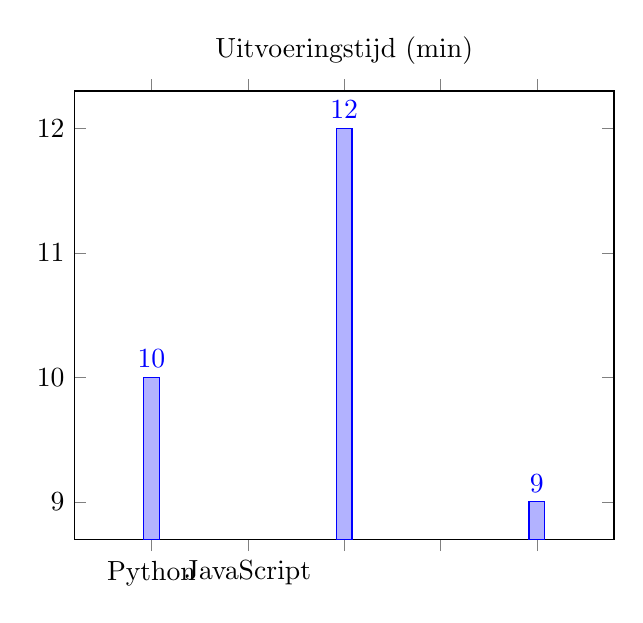
\begin{tikzpicture}
\begin{axis}[
  title=Uitvoeringstijd (min),
  ybar,
  nodes near coords,
  bar width=0.2cm,
  symbolic x coords={Java,Python,Javascript},
  enlarge x limits=.2,
  xticklabels={Java,Python,JavaScript},
]

\addplot coordinates {
  (Java,10)
  (Python,12)
  (Javascript,9)
};

\end{axis}
\end{tikzpicture}
  
Een aanvullend aspect van de verwachte resultaten omvat de beoordeling van codecomplexiteit en praktische bruikbaarheid in webscraping
-implementaties voor elke taal.

De meerwaarde van dit onderzoek voor de doelgroep ligt in de mogelijkheid om optimalere technologische keuzes te maken. 
Door inzicht te verschaffen in de prestaties van Python, JavaScript en Java, biedt dit onderzoek een waardevolle leidraad. 